% !TeX root = ../main.tex

\section{Introduction}
The idea of the recursive nearest neighbors method came up in the process of studying
recommender systems in the framework of this thesis. The method that will be presented is an
effort to overcome the limitations of neighborhood-based approach. That is, to provide more
rating predictions than the conventional K-Nearest Neighbors method, which fails when it
cannot connect users or items directly due to sparseness constraints.

\begin{table}[H]
\centering
\begin{tabular}{ |c|c|c|c|c|c|c| }
\hline
\diagbox{$User$}{$Item$} & \textbf{$Item_1$} & \textbf{$Item_2$} & \textbf{$Item_3$} & \textbf{$Item_4$}  & \textbf{$Item_5$} & \textbf{$Item_6$} \\
\hline
\textbf{$User_1$} & 5 & 2 & 3 & \textbf{?} & 1 & 5 \\
\hline
\textbf{$User_2$} & 1 & 2 & 4 & \textbf{?} & 2 & 2 \\
\hline
\textbf{$User_3$} & 4  & 3 & 5 & \textbf{?} & 4 & 3 \\
\hline
\textbf{$User_4$} & 5 & 2 & 3 &  \textbf{?} & \textbf{?} & \textbf{?} \\
\hline
\textbf{$User_5$} & \textbf{?} & \textbf{?}  & \textbf{?} & 4 & 1 & 1 \\
\hline
\textbf{$User_6$} & \textbf{?} & \textbf{?} & \textbf{?}  & 3 & 5 & 2 \\
\hline
\textbf{$User_7$} & \textbf{?} & \textbf{?} & \textbf{?}  & 5 & 1 & 2 \\
\hline
\textbf{$User_8$} & \textbf{?} & \textbf{?} & \textbf{?}  & 5 & 4 & 4 \\
\hline
\end{tabular}
\caption{Modified Ratings Matrix}
\label{table:Modified Ratings Matrix}
\end{table}

The above table is a modification/extension of \autoref{table:Ratings Matrix}. If KNN was applied to
this rating matrix with $\mathcal{K}=4$(all users do not have 4 available NN, instead
they use the largest amount of NN available to them before 4) using user cosine similarity,
it would produce the rating predictions in the table below.

\begin{table}[H]
\centering
\begin{tabular}{ |c|c|c|c|c|c|c| }
\hline
\diagbox{$User$}{$Item$} & \textbf{$Item_1$} & \textbf{$Item_2$} & \textbf{$Item_3$} & \textbf{$Item_4$}  & \textbf{$Item_5$} & \textbf{$Item_6$} \\
\hline
\textbf{$User_1$} & 5 & 2 & 3 & {\color{red}4.3} & 1 & 5 \\
\hline
\textbf{$User_2$} & 1 & 2 & 4 & {\color{red}4.15} & 2 & 2 \\
\hline
\textbf{$User_3$} & 4  & 3 & 5 & {\color{red}4.12} & 4 & 3 \\
\hline
\textbf{$User_4$} & 5 & 2 & 3 &  {\color{green}\textbf{?}} & {\color{red}2.35} & {\color{red}3.42} \\
\hline
\textbf{$User_5$} & {\color{red}3.35} & {\color{red}2.35}  & {\color{red}4.02} & 4 & 1 & 1 \\
\hline
\textbf{$User_6$} & {\color{red}3.21} & {\color{red}2.4} & {\color{red}4.15}  & 3 & 5 & 2 \\
\hline
\textbf{$User_7$} & {\color{red}3.46} & {\color{red}2.32} & {\color{red}3.94}  & 5 & 1 & 2 \\
\hline
\textbf{$User_8$} & {\color{red}3.36} & {\color{red}2.35} & {\color{red}4.03}  & 5 & 4 & 4 \\
\hline
\end{tabular}
\caption{Modified Ratings Matrix After KNN}
\label{table:Modified Ratings Matrix after KNN}
\end{table}
\justify
It seems that KNN was unable to predict how $User_4$ would rate $Item_4$.\\
The connections from user cosine similarity that could be formed were the following:
\begin{align*}
	&cos(User_1,User_2) = 0.7659 &cos(User_1,User_3) = 0.8660 & &cos(User_1,User_4) = 0.7705\\
	&cos(User_1,User_5) = 0.1767 &cos(User_1,User_6) = 0.3041 & &cos(User_1,User_7) = 0.2510\\
	&cos(User_1,User_8) = 0.3973 &cos(User_2,User_3) = 0.9434 & &cos(User_2,User_4) = 0.6325\\
	&cos(User_2,User_5) = 0.1750 &cos(User_2,User_6) = 0.4217 & &cos(User_2,User_7) = 0.2034\\
	&cos(User_2,User_8) = 0.3935 &cos(User_3,User_4) = 0.7680 & &cos(User_3,User_5) = 0.1905\\
	&cos(User_3,User_6) = 0.4870 &cos(User_3,User_7) = 0.2108 & &cos(User_3,User_8) = 0.4282\\
	&cos(User_5,User_6) = 0.7264 &cos(User_5,User_7) = 0.9897 & &cos(User_5,User_8) = 0.8741\\
	&cos(User_6,User_7) = 0.7108 &cos(User_6,User_8) = 0.9239 & &cos(User_7,User_8) = 0.8947\\
\end{align*}
\vfill
\justify
The following figure is a graphical representation of the user connections.
\begin{figure}[H]
\centering
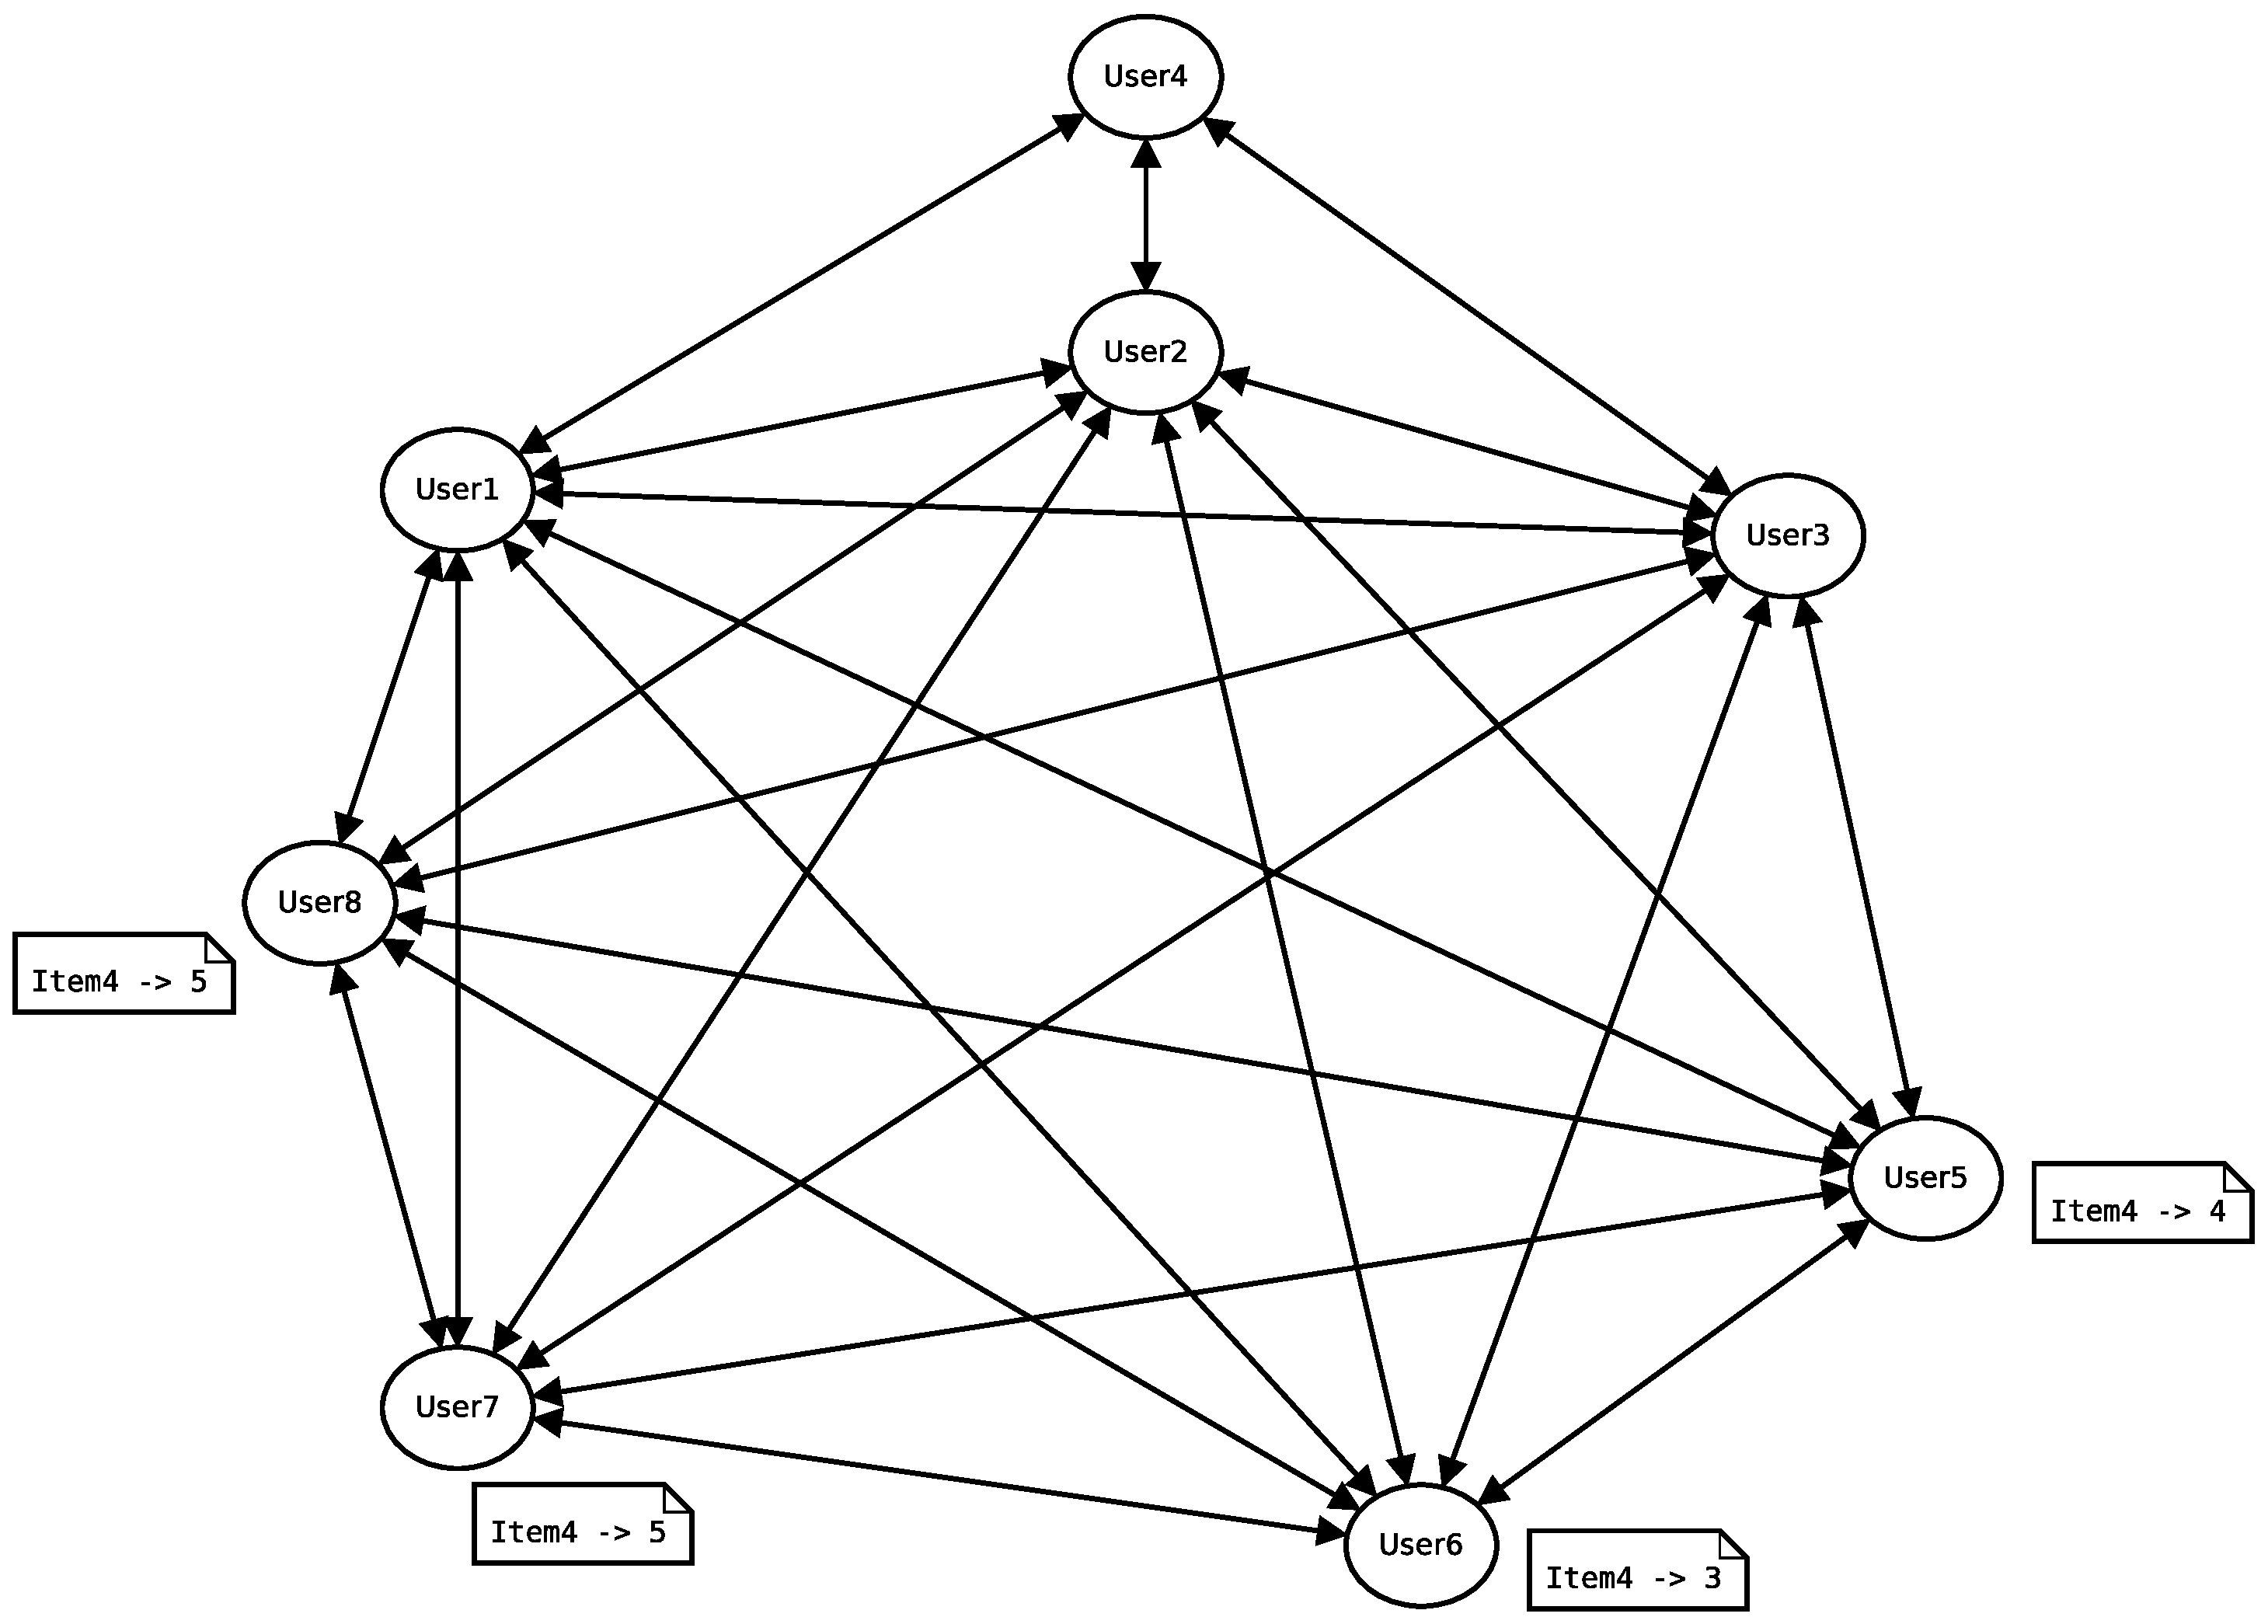
\includegraphics[width=0.8\textwidth]{chapter_3/user_connections.eps}
\caption{User Connections}
\label{figure:user_connections}
\end{figure}

It seems that from users who have rated $Item_4$, it is possible to create a connection to $User_4$, but in
order to do that they must use the intermediate connections they have in common. Graph-based
methods are known to utilize these connections efficiently to produce link similarities that
surpass the direct connection between users or items \citep{Ricci,Aggarwal}.
\section{Methodology}
The Recursive K-Nearest Neighbors algorithm utilizes the intermediate connections that two users
have in common in order to find a path to predict ratings that the conventional KNN could not find.
The concept of this algorithm, is to use the rating predictions produced by KNN, in order
to consider the users that have not rated the target item, as neighbors. As presented in
\autoref{figure:user_connections_with_KNN} below,
the KNN rating predictions related to $Item_4$ for $User_1$, $User_2$ and $User_3$ have been
added to the figure to indicate them as real rating values that these users gave to $Item_4$.
\begin{figure}[H]
\centering
\includegraphics[width=0.8\textwidth]{chapter_3/user_connections_with_KNN.eps}
\caption{User Connections as \autoref{figure:user_connections} with KNN predictions from \autoref{table:Modified Ratings Matrix after KNN}}
\label{figure:user_connections_with_KNN}
\end{figure}
Then, as new similarities can be formed for $User_4$ with $User_1$, $User_2$ and $User_3$ for $Item_4$, the weighted sum formula used in KNN can be
again used to compute the rating prediction of $User_4$ to $Item_4$ as shown in \autoref{figure:RKNN_prediction}.\\
\begin{figure}[H]
\centering
\includegraphics[width=0.8\textwidth]{chapter_3/RKNN_prediction.eps}
\caption{Recursive KNN Rating Prediction}
\label{figure:RKNN_prediction}
\end{figure}
The Recursive K-Nearest Neighbors methodology for predicting how $User_A$ would rate $Item_B$,
(with the assumption that, given a similarity metric, KNN would not be able to predict this rating)
consists of the following steps:
\begin{itemize}\label{RKNN}
	\item[] \textbf{Step 1:} Select users that are connected with $User_A$, and name it $Group_A$.
	\item[] \textbf{Step 2:} Out of $Group_A$, choose those users that have connections with
	users who have rated $Item_B$, and name it $Group_B$.
	\item[] \textbf{Step 3:}  Order $Group_B$ by descending similarity with $User_A$.
	\item[] \textbf{Step 4:}  Choose how many neighbors from $Group_B$ will contribute in the
	rating prediction by selecting the top $\mathcal{K}$ out of all the available
	neighbors in this group, and name it $Group_C$.
	\item[] \textbf{Step 5:} For each neighbor in $Group_C$, predict how this neighbor would
	rate $Item_B$ using the KNN algorithm. For convenience, we name the number of recursive
	neighbors each neighbor in $Group_C$ uses as, $\mathcal{M}$-Nearest Neighbors.
	\item[] \textbf{Step 6:} Use the rating predictions applied on $Group_C$ to perform
	the KNN algorithm on $User_A$ for $Item_B$.
\end{itemize}

Now that the steps for performing the Recursive K-Nearest Neighbors algorithm have been
introduced let us look at a general case as in the figure below:\\
\begin{figure}[H]
\centering
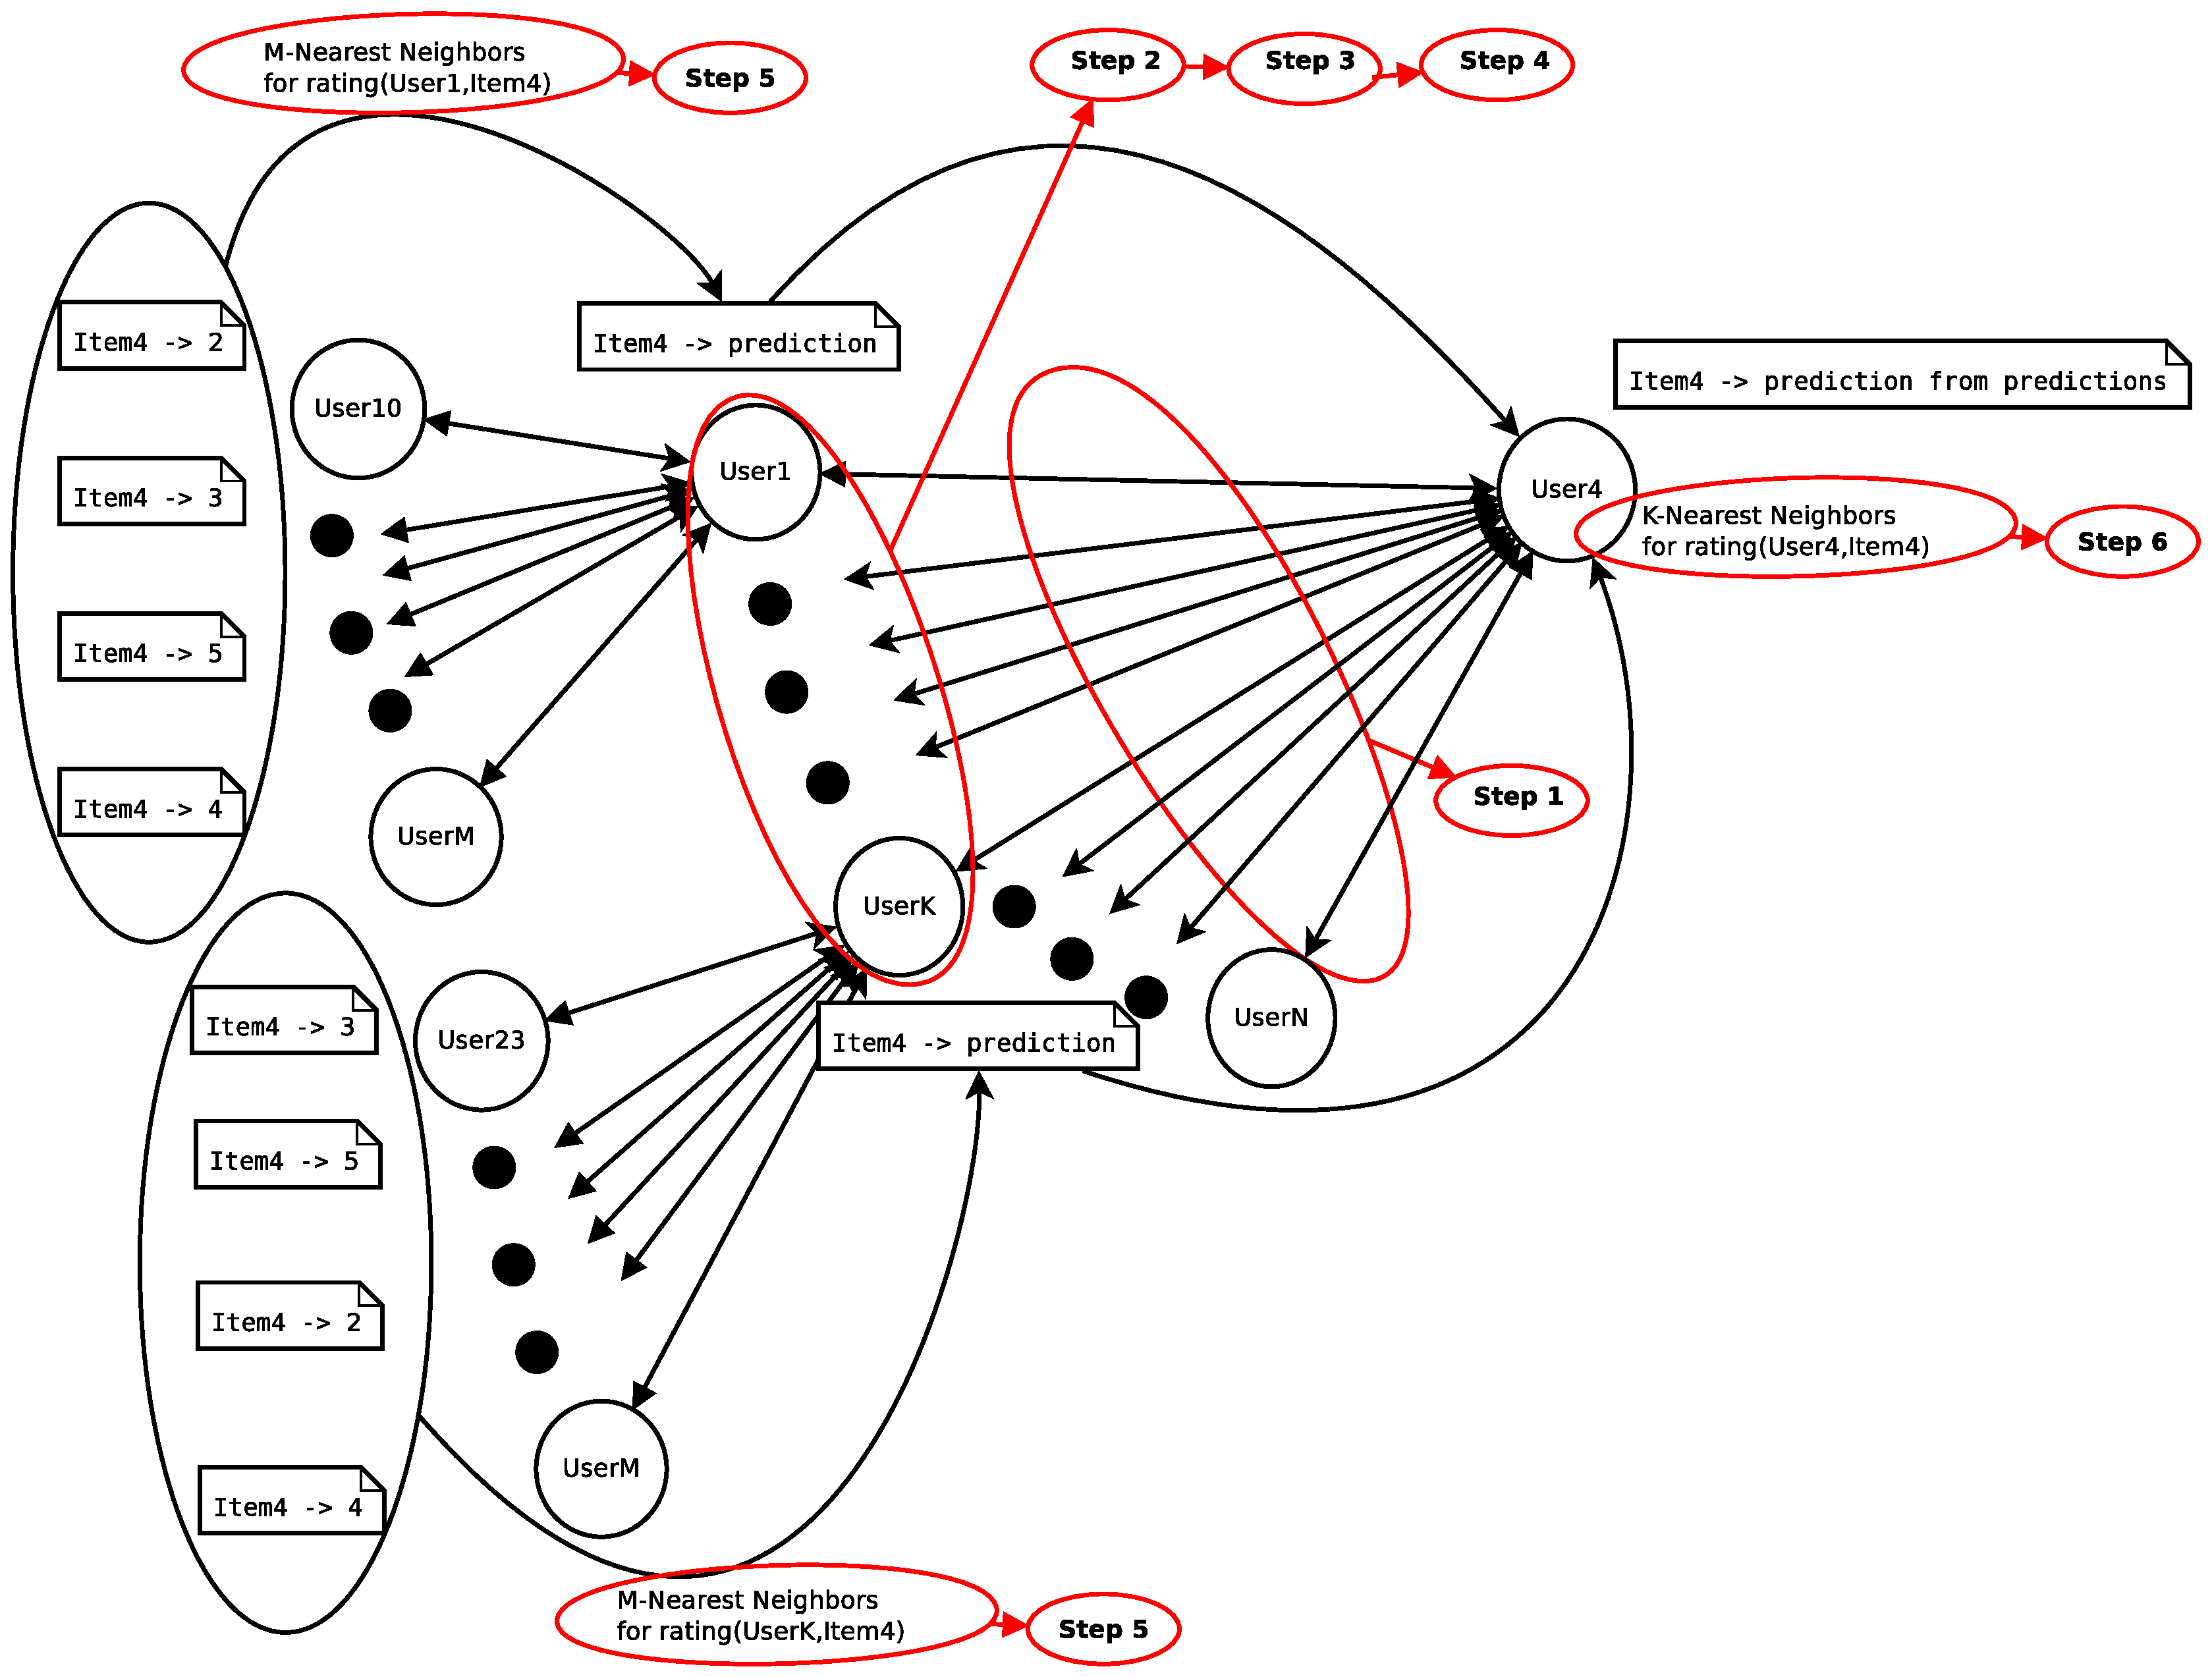
\includegraphics[width=0.8\textwidth]{chapter_3/Recursive_Nearest_Neighbors.eps}
\caption{Recursive Nearest Neighbors Algorithm}
\label{figure:recursive_algorithm}
\end{figure}
Interpretation of the figure:
\begin{enumerate}
	\item After the selection of the top $\mathcal{K}$ relevant Neighbors.
	(\textbf{Steps 1,2,3,4})
	\item For each Neighbor, name it $Neighbor_i$, out of $\mathcal{K}$'s choose $\mathcal{M}$
	Neighbors to apply KNN on $Neighbor_i$. (\textbf{Step 5})
	\item Use the rating predictions applied on $\mathcal{K}$'s to predict the requested
	User-Item rating.\\ (\textbf{Step 6})
\end{enumerate}
